\documentclass[a4paper,english,12pt]{article}
\usepackage{%
	amsmath,%
	amsfonts,%
	amssymb,%
	amsthm,%
	hyperref,%
	url,%
	latexsym,%
	epsfig,%
	graphicx,%
	psfrag,%
	subfigure,%	
	color,%
	tikz,%
	pgf,%
	pgfplots,%
	pgfplotstable,%
	pgfpages,%
	proofs%
}

\usepgflibrary{shapes}
\usetikzlibrary{%
  arrows,%
	backgrounds,%
	chains,%
	decorations.pathmorphing,% /pgf/decoration/random steps | erste Graphik
	decorations.text,%
	matrix,%
  positioning,% wg. " of "
  fit,%
	patterns,%
  petri,%
	plotmarks,%
  scopes,%
	shadows,%
  shapes.misc,% wg. rounded rectangle
  shapes.arrows,%
	shapes.callouts,%
  shapes%
}

\theoremstyle{plain}
\newtheorem{thm}{Theorem}[section]
\newtheorem{lem}[thm]{Lemma}
\newtheorem{prop}[thm]{Proposition}
\newtheorem{cor}[thm]{Corollary}

\theoremstyle{definition}
\newtheorem{defn}[thm]{Definition}
\newtheorem{conj}[thm]{Conjecture}
\newtheorem{exmp}[thm]{Example}
\newtheorem{assum}[thm]{Assumptions}

%\theoremstyle{remark}
\newtheorem{rem}{Remark}
\newtheorem{note}{Note}

\makeatletter
\def\th@plain{%
  \thm@notefont{}% same as heading font
  \itshape % body font
}
\def\th@definition{%
  \thm@notefont{}% same as heading font
  \normalfont % body font
}
\makeatother
\date{}

%opening
\title{Lecture 15: The subspace topology, Closed sets}
\author{}

\begin{document}
\maketitle

\section{The Subspace Topology}
\begin{defn}
	Let $(X,\mathcal{T})$ be a topological space with topology $\mathcal{T}$. If $Y$ is a subset of $X$, the collection 
	\[ \mathcal{T}_Y = \{Y \cap U | U \in \mathcal{T}\}	\]
	is a topology on $Y$, called the \textbf{subspace topology}. With this topology, $Y$ is called a \textbf{subspace} of $X$; its open sets consist of alt intersections of open sets of $X$ with $Y$.
\end{defn}
Check that $\mathcal{T}_Y$ is a topology: 
\begin{enumerate}
	\item It contains $\phi$ and $Y$ because 
	\[  \phi = Y \cap \phi \, and \, Y = Y \cap X.\]
	where $\phi$ and $X$ are elements of $\mathcal{T}$.	
	\item It is closed under finite intersections:
	\[ (U_1 \cap Y) \cap ... \cap (U_n \cap Y) = (U_1 \cap ... \cap U_n) \cap Y. \]	
	\item It is closed under arbitrary unions:
	\[ \bigcup_{\alpha \in J} (U_\alpha \cap Y) = (\bigcup_{\alpha \in J}U_\alpha) \cap Y.\]
\end{enumerate}

\begin{lem}
	Let $\mathcal{B}$ be a basis for the topology of $X$ then the collection
	\[ \mathcal{B}_Y = \{B \cap Y | B \in \mathcal{B\}} \]
	is a basis for the subspace topology on $Y$.
\end{lem}

\begin{proof}
	Given $U$ open in $X$ and given $y \in U \cap Y$, we can choose an element $B$ of $\mathcal{B}$ such that $y \in B \subset U$. Then $y \in B \cap Y \subset U \cap Y$. It follows from Lemma 13.2 that $\mathcal{B}_Y$ is a basis for the subspace topology on $Y$.
\end{proof}

When dealing with a space $X$ and a subspace $Y$, one needs to be careful when
one uses the term \lq \lq open set". Does one mean an element of the topology of $Y$ or an element of the topology of $X$? We make the following definition:

\begin{defn}
	If $Y$ is a subspace of $X$, we say that a set $U$ is \textbf{open in $Y$} if $U \in \mathcal{T}_Y$; this implies in particular that it is a subset of $Y$. We say that $U$ is \textbf{open in $X$} if $U \in \mathcal{T}_X$.
\end{defn} 

\begin{lem}
	Let $Y$ be a subspace of $X$. If $U$ is open in $Y$ and $Y$ is open in $X$, then $U$ is open in $X$.
\end{lem}
\begin{proof}
	Since $U$ is open in $Y$, $U = Y \cap V$ for some set $V$ open in $X$. Since $Y$ and $V$ are both open in $X$, so is $Y \cap V$.
\end{proof}

In the following theorem, the relation between the subspace topology and the order and product topologies has been discussed.

\begin{thm}
	If $A$ is a subspace of $X$ and $B$ is a subspace of $Y$, then the product
	topology on $A \times B$ is the same as the topology $A \times B$ inherits as a subspace of $X \times Y$.
\end{thm}

\begin{proof}
	The set $U \times V$ is the general basis element for $X \times Y$, where $U$ is open in $X$ and $V$ is open in $Y$. Therefore, $(U \times V) \cap (A \times B)$ is the general basis element for the subspace topology on $A \times B$. Now,
	\[ (U \times V) \cap (A \times B) = (U \cap A) \times (V \cap B). \]
	Since $U \cap A$ and $V \times B$ are the general open sets for the subspace topologies on $A$ and $B$, respectively, the set $(U \cap A) \times (V \cap B)$ is the general basis element for the product topology on $A \times B$.
	Hence, we can conclude that the bases for the subspace topology on $A \times B$ and for the product topology on $A \times B$ are the same. Hence the topologies are the same.
\end{proof}

Now, let $X$ be an ordered set in the order topology, and let $Y$ be a subset of $X$. The order relation on $X$, when restricted to $Y$, makes $Y$ into an ordered set. However, \textit{the resulting order topology on $Y$ need not be the same as the topology that $Y$ inherits as a subspace of $X$.} \\
Consider the following examples:

\begin{exmp}
	Consider the subset $Y = [0,1] \subseteq \mathbb{R}$, in the subspace topology. The subspace topology has as basis $\mathcal{B}=\{(a,b) \cap Y | (a,b) \, is\, an\, open\, interval\, in\, \mathbb{R}\}$. Such a set is of one of the following types.
	\[ (a,b)\cap Y = 
		\begin{dcases*}
	(a,b) & if  $a,b \in Y$\\
	[a,b) & if  $a \notin Y, b \in Y$\\
	(a,1] & if  $b \notin Y, a \in Y$\\
	Y \, or \, \phi & if  $b \notin Y, a \notin Y$\\
		\end{dcases*}  
	\]
	
	By definition, each of these sets is open in $Y$. But sets of the second and third types are not open in the larger space $\mathbb{R}$.\\ 
	\textbf{Note}: These sets form a basis for the order topology on $Y$. Thus, we see that in the case of the set $Y = [0,1]$, its subspace topology and its order topology are the same.
\end{exmp}

\begin{exmp}
	Let $Y$ be the subset $[0, 1) \cup \{2\} \in \mathbb{R}$. In the subspace topology on $Y$ the	one-point set $\{2\}$ is open, because $\{2\} = (\frac{3}{2} , \frac{5}{2} ) \cap Y$. But in the order topology on $Y$, the set $\{2\}$ is not open. Any basis element for the order topology 	on $Y$ that contains $2$ is of the form
	
	\[ \{ x | x \in Y \, and \, a < x \leq 2 \} \]
	for some $a \in Y$, such a set necessarily contains points of $Y$ less than $2$.
\end{exmp}

\begin{exmp}
	Let $I = [0,1]$. The dictionary order on $I \times I$ is just the restriction to $I \times I$ of the dictionary order on the plane $\mathbb{R} \times \mathbb{R}$. However, the dictionary order topology
	on $I \times I$ is not the same as the subspace topology on $I \times I$ obtained from the dictionary order topology on $\mathbb{R} \times \mathbb{R}$. \\
	For example, the set $\{l/2\} \times (1/2, 1]$ is open in $I \times I$ in the subspace topology, but not in the order topology. See Figure \ref{fig1}.
	
\end{exmp}

\begin{figure}
	\centering
	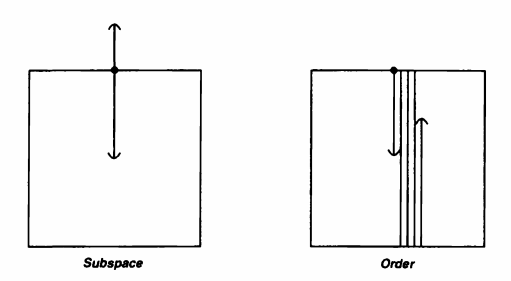
\includegraphics[width=0.8\linewidth]{Figures/Lecture15_Fig1}
	\caption{Subspace and order}
	\label{fig1}
\end{figure}

\begin{defn}
	The set $I \times I$ in the dictionary order topology is called the \textbf{ordered square}, and is denoted by $I_0^2$.
\end{defn}

The anomaly seen in Examples 2 and 3 does not occur for intervals or rays in an ordered set $X$.
\begin{defn}
	Given an ordered set $X$, let us say that a subset $Y$ of $X$ is convex in $X$ if for each pair of points $a < b$ of $Y$, the entire interval $(a,b)$ of points of $X$ lies in $Y$. 
\end{defn}
\textbf{Note}: Intervals and rays in $X$ are convex in $X$.

\begin{thm}
	Let $X$ be an ordered set in the order topology, let $Y$ be a subset
	of $X$ that is convex in $X$. Then the order topology on $Y$ is the same as the topology $Y$	inherits as a subspace of $X$.
\end{thm}

\begin{proof}
	Consider the ray $(a, +\infty)$ in $X$. If $a \in Y$, then
	\[(a, +\infty) \cap Y = 
		\begin{dcases*}
			\{x : x \in Y , x > a\} & a $\in$ Y\\
			Y & a=lower bound on Y, a $\notin$ Y\\
			\phi  & a=upper bound on Y, a $\notin$ Y
		\end{dcases*}
	\]
	
		A similar remark shows that the intersection of the ray $(—\infty, a)$ with $Y$ is either	an open ray of $Y$, or $Y$ itself, or empty. Since the sets $(a, +\infty) \cap Y$ and $(-\infty,a \cap Y)$ form a sub-basis for the subspace topology on $Y$, and since each is open in the order topology, the order topology contains the subspace topology.\\
		To prove the reverse, note that any open ray of $Y$ equals the intersection of an open ray of $X$ with $Y$, so it is open in the subspace topology on $Y$. Since the open rays of $Y$ are a sub-basis for the order topology on $Y$, this topology is contained in the subspace topology.
\end{proof}

\section{Closed Sets}
Some of the basic concepts associated with topological spaces such as closed set, closure of a set and limit point will be discussed.

\begin{defn}[Closed set]
	A subset $A$ of a topological space $X$ is said to be closed if the set $X - A$ is open.
\end{defn}
	
\begin{exmp}
	The closed interval $[a,b] \subseteq \mathbb{R}$ is closed.because its complement $\mathbb{R}-[a,b] = (-\infty,a) \cup (b,+\infty)$ is open.\\
	Similarly, closed rays $[a,+\infty) \subseteq \mathbb{R}$ and $(-\infty,a] \subseteq \mathbb{R}$ are closed.\\
	The subset $[a,b)$ of $\mathbb{R}$ is neither open nor closed.
\end{exmp}

\begin{exmp}
	In the plane $\mathbb{R}^2$, the set $\{x \times y | x \geq 0 \, and \, y \geq 0\}$ is closed, because its complement is the union of the two sets
	$(—\infty, 0) \times \mathbb{R}$ and $\mathbb{R} \times (-\infty,0)$,
	each of which is a product of open sets of $\mathbb{R}$ and is, therefore, open in $\mathbb{R}^2$.
\end{exmp}
	
	
\begin{exmp}
	In the finite complement topology on a set $X$, the closed sets consist of $X$ itself and all finite subsets of $X$.
\end{exmp}

\begin{exmp}
	In the discrete topology on the set $X$, every set is open, it follows that every set is closed as well.	
\end{exmp}

\begin{exmp}
	Consider the following subset of the real line:
	$Y=[0, 1]\cup(2,3)$,
	in the subspace topology. In this space, the set $[0, 1]$ is open, since it is the intersection of the open set $(—1/2, 3/2)$ of $\mathbb{R}$ with $Y$. Similarly, $(2, 3)$ is open as a subset of $Y$; it is even open
	as a subset of $\mathbb{R}$. Since $[0, 1]$ and $(2, 3)$ are complements in $Y$ of each other, we conclude that both $[0, 1]$ and $(2, 3)$ are closed as subsets of $Y$.
\end{exmp}
		
The collection of closed subsets of a space $X$ has properties similar to those satisfied by the collection of open subsets of $X$:

\begin{thm}
	Let $X$ be a topological space. Then the following conditions hold:
	\begin{enumerate}
		\item $\phi$ and $X$ are closed.
		\item Arbitrary intersections of closed sets are closed.
		\item Finite unions of closed sets are closed.
	\end{enumerate}
\end{thm}

\begin{proof}
	\begin{enumerate}
		\item $\phi$ and $X$ are closed because they are the complements of the open sets $X$ and $\phi$, respectively.
		
		\item Given a collection of closed sets we apply De Morgan's law,
		\begin{align*}
			X \setminus\bigcap_{\alpha \in J} A_\alpha = \bigcup_{\alpha \in J} (X \setminus A_\alpha).
		\end{align*}
		Since the sets $X \setminus A_\alpha$ are open by definition, the right side of this equation represents	an arbitrary union of open sets, and is thus open. Therefore, $\bigcap A_\alpha$ is closed.
		
		\item Similarly, if $A_i$ is closed for $i \in [n]$, consider the equation
		\begin{align*}
			X \setminus\bigcup_{\alpha \in J}^n A_i = \bigcap_{\alpha \in J}^n (X \setminus A_i).
		\end{align*}
		The set on the right side of this equation is a finite intersection of open sets and is therefore open. Hence $\cup A_i$ is closed.
	\end{enumerate}
\end{proof}
	
	
\end{document}